\documentclass{standalone}
\usepackage{tikz}
\usetikzlibrary{patterns, positioning}


\begin{document}
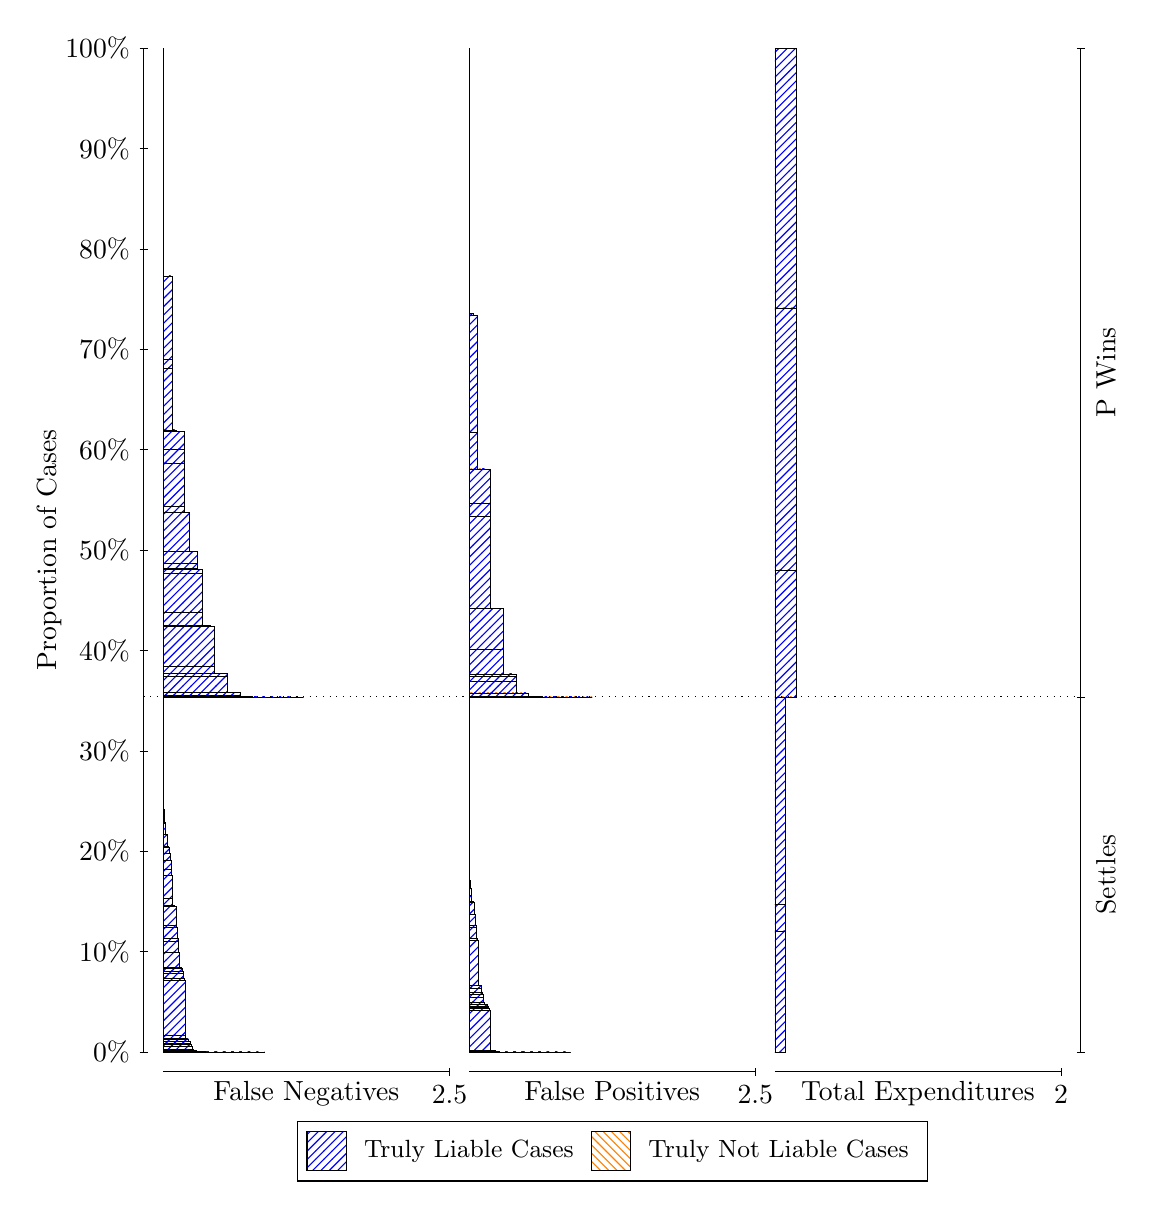
\begin{tikzpicture}
\draw[black, very thin] (1.5,1.75) -- (1.5,14.5);
\node[rotate=90, text=black, anchor=center] at (0.3, 8.125) {Proportion of Cases};
\draw[black, very thin] (1.45,1.75) -- (1.55,1.75);
\node[text=black, anchor=east] at (1.45, 1.75) {0\%};
\draw[black, very thin] (1.45,3.025) -- (1.55,3.025);
\node[text=black, anchor=east] at (1.45, 3.025) {10\%};
\draw[black, very thin] (1.45,4.3) -- (1.55,4.3);
\node[text=black, anchor=east] at (1.45, 4.3) {20\%};
\draw[black, very thin] (1.45,5.575) -- (1.55,5.575);
\node[text=black, anchor=east] at (1.45, 5.575) {30\%};
\draw[black, very thin] (1.45,6.85) -- (1.55,6.85);
\node[text=black, anchor=east] at (1.45, 6.85) {40\%};
\draw[black, very thin] (1.45,8.125) -- (1.55,8.125);
\node[text=black, anchor=east] at (1.45, 8.125) {50\%};
\draw[black, very thin] (1.45,9.4) -- (1.55,9.4);
\node[text=black, anchor=east] at (1.45, 9.4) {60\%};
\draw[black, very thin] (1.45,10.675) -- (1.55,10.675);
\node[text=black, anchor=east] at (1.45, 10.675) {70\%};
\draw[black, very thin] (1.45,11.95) -- (1.55,11.95);
\node[text=black, anchor=east] at (1.45, 11.95) {80\%};
\draw[black, very thin] (1.45,13.225) -- (1.55,13.225);
\node[text=black, anchor=east] at (1.45, 13.225) {90\%};
\draw[black, very thin] (1.45,14.5) -- (1.55,14.5);
\node[text=black, anchor=east] at (1.45, 14.5) {100\%};

\draw[black, very thin] (13.4,1.75) -- (13.4,14.5);
\draw[black, very thin] (13.35,1.75) -- (13.45,1.75);
\node[anchor=west] at (13.35, 1.75) {};
\draw[black, very thin] (13.35,6.2598) -- (13.45,6.2598);
\node[anchor=west] at (13.35, 6.2598) {};
\draw[black, very thin] (13.35,14.5) -- (13.45,14.5);
\node[anchor=west] at (13.35, 14.5) {};

\draw[black, very thin, pattern color=blue, pattern=north east lines] (1.75,1.75) rectangle (3.0398,1.75);
\draw[black, very thin, pattern color=blue, pattern=north east lines] (1.75,1.75) rectangle (2.9672,1.75);
\draw[black, very thin, pattern color=blue, pattern=north east lines] (1.75,1.75) rectangle (2.8945,1.75);
\draw[black, very thin, pattern color=blue, pattern=north east lines] (1.75,1.75) rectangle (2.8784,1.75);
\draw[black, very thin, pattern color=blue, pattern=north east lines] (1.75,1.75) rectangle (2.8218,1.75);
\draw[black, very thin, pattern color=blue, pattern=north east lines] (1.75,1.75) rectangle (2.8057,1.75);
\draw[black, very thin, pattern color=blue, pattern=north east lines] (1.75,1.75) rectangle (2.7492,1.75);
\draw[black, very thin, pattern color=blue, pattern=north east lines] (1.75,1.75) rectangle (2.733,1.75);
\draw[black, very thin, pattern color=blue, pattern=north east lines] (1.75,1.75) rectangle (2.7169,1.75);
\draw[black, very thin, pattern color=blue, pattern=north east lines] (1.75,1.75) rectangle (2.6765,1.75);
\draw[black, very thin, pattern color=blue, pattern=north east lines] (1.75,1.75) rectangle (2.6604,1.75);
\draw[black, very thin, pattern color=blue, pattern=north east lines] (1.75,1.75) rectangle (2.6442,1.75);
\draw[black, very thin, pattern color=blue, pattern=north east lines] (1.75,1.75) rectangle (2.6038,1.75);
\draw[black, very thin, pattern color=blue, pattern=north east lines] (1.75,1.75) rectangle (2.5877,1.75);
\draw[black, very thin, pattern color=blue, pattern=north east lines] (1.75,1.75) rectangle (2.5715,1.75);
\draw[black, very thin, pattern color=blue, pattern=north east lines] (1.75,1.75) rectangle (2.5554,1.75);
\draw[black, very thin, pattern color=blue, pattern=north east lines] (1.75,1.75) rectangle (2.5312,1.75);
\draw[black, very thin, pattern color=blue, pattern=north east lines] (1.75,1.75) rectangle (2.515,1.75);
\draw[black, very thin, pattern color=blue, pattern=north east lines] (1.75,1.75) rectangle (2.4989,1.75);
\draw[black, very thin, pattern color=blue, pattern=north east lines] (1.75,1.75) rectangle (2.4827,1.75);
\draw[black, very thin, pattern color=blue, pattern=north east lines] (1.75,1.75) rectangle (2.4585,1.75);
\draw[black, very thin, pattern color=blue, pattern=north east lines] (1.75,1.75) rectangle (2.4424,1.75);
\draw[black, very thin, pattern color=blue, pattern=north east lines] (1.75,1.75) rectangle (2.4262,1.75);
\draw[black, very thin, pattern color=blue, pattern=north east lines] (1.75,1.75) rectangle (2.4101,1.75);
\draw[black, very thin, pattern color=blue, pattern=north east lines] (1.75,1.75) rectangle (2.3939,1.75);
\draw[black, very thin, pattern color=blue, pattern=north east lines] (1.75,1.75) rectangle (2.3858,1.75);
\draw[black, very thin, pattern color=blue, pattern=north east lines] (1.75,1.75) rectangle (2.3697,1.75);
\draw[black, very thin, pattern color=blue, pattern=north east lines] (1.75,1.75) rectangle (2.3535,1.7501);
\draw[black, very thin, pattern color=blue, pattern=north east lines] (1.75,1.7501) rectangle (2.3374,1.7501);
\draw[black, very thin, pattern color=blue, pattern=north east lines] (1.75,1.7501) rectangle (2.3212,1.7502);
\draw[black, very thin, pattern color=blue, pattern=north east lines] (1.75,1.7502) rectangle (2.3132,1.7502);
\draw[black, very thin, pattern color=blue, pattern=north east lines] (1.75,1.7502) rectangle (2.297,1.7503);
\draw[black, very thin, pattern color=blue, pattern=north east lines] (1.75,1.7503) rectangle (2.2809,1.7526);
\draw[black, very thin, pattern color=blue, pattern=north east lines] (1.75,1.7526) rectangle (2.2647,1.7533);
\draw[black, very thin, pattern color=blue, pattern=north east lines] (1.75,1.7533) rectangle (2.2486,1.7538);
\draw[black, very thin, pattern color=blue, pattern=north east lines] (1.75,1.7538) rectangle (2.2405,1.7539);
\draw[black, very thin, pattern color=blue, pattern=north east lines] (1.75,1.7539) rectangle (2.2324,1.7545);
\draw[black, very thin, pattern color=blue, pattern=north east lines] (1.75,1.7545) rectangle (2.2244,1.7546);
\draw[black, very thin, pattern color=blue, pattern=north east lines] (1.75,1.7546) rectangle (2.2082,1.7547);
\draw[black, very thin, pattern color=blue, pattern=north east lines] (1.75,1.7547) rectangle (2.1921,1.7595);
\draw[black, very thin, pattern color=blue, pattern=north east lines] (1.75,1.7595) rectangle (2.1759,1.7615);
\draw[black, very thin, pattern color=blue, pattern=north east lines] (1.75,1.7615) rectangle (2.1678,1.7712);
\draw[black, very thin, pattern color=blue, pattern=north east lines] (1.75,1.7712) rectangle (2.1598,1.7731);
\draw[black, very thin, pattern color=blue, pattern=north east lines] (1.75,1.7731) rectangle (2.1517,1.7752);
\draw[black, very thin, pattern color=blue, pattern=north east lines] (1.75,1.7752) rectangle (2.1355,1.7781);
\draw[black, very thin, pattern color=blue, pattern=north east lines] (1.75,1.7781) rectangle (2.1194,1.8264);
\draw[black, very thin, pattern color=blue, pattern=north east lines] (1.75,1.8264) rectangle (2.1032,1.8499);
\draw[black, very thin, pattern color=blue, pattern=north east lines] (1.75,1.8499) rectangle (2.0952,1.8647);
\draw[black, very thin, pattern color=blue, pattern=north east lines] (1.75,1.8647) rectangle (2.0871,1.8864);
\draw[black, very thin, pattern color=blue, pattern=north east lines] (1.75,1.8864) rectangle (2.079,1.8898);
\draw[black, very thin, pattern color=blue, pattern=north east lines] (1.75,1.8898) rectangle (2.0709,1.9155);
\draw[black, very thin, pattern color=blue, pattern=north east lines] (1.75,1.9155) rectangle (2.0629,1.9175);
\draw[black, very thin, pattern color=blue, pattern=north east lines] (1.75,1.9175) rectangle (2.0467,1.9193);
\draw[black, very thin, pattern color=blue, pattern=north east lines] (1.75,1.9193) rectangle (2.0306,1.9676);
\draw[black, very thin, pattern color=blue, pattern=north east lines] (1.75,1.9676) rectangle (2.0225,2.6586);
\draw[black, very thin, pattern color=blue, pattern=north east lines] (1.75,2.6586) rectangle (2.0144,2.6906);
\draw[black, very thin, pattern color=blue, pattern=north east lines] (1.75,2.6906) rectangle (2.0064,2.7472);
\draw[black, very thin, pattern color=blue, pattern=north east lines] (1.75,2.7472) rectangle (1.9983,2.7797);
\draw[black, very thin, pattern color=blue, pattern=north east lines] (1.75,2.7797) rectangle (1.9902,2.8088);
\draw[black, very thin, pattern color=blue, pattern=north east lines] (1.75,2.8088) rectangle (1.9741,2.8272);
\draw[black, very thin, pattern color=blue, pattern=north east lines] (1.75,2.8272) rectangle (1.9579,3.0202);
\draw[black, very thin, pattern color=blue, pattern=north east lines] (1.75,3.0202) rectangle (1.9418,3.1616);
\draw[black, very thin, pattern color=blue, pattern=north east lines] (1.75,3.1616) rectangle (1.9337,3.195);
\draw[black, very thin, pattern color=blue, pattern=north east lines] (1.75,3.195) rectangle (1.9256,3.3336);
\draw[black, very thin, pattern color=blue, pattern=north east lines] (1.75,3.3336) rectangle (1.9175,3.3538);
\draw[black, very thin, pattern color=blue, pattern=north east lines] (1.75,3.3538) rectangle (1.9095,3.5976);
\draw[black, very thin, pattern color=blue, pattern=north east lines] (1.75,3.5976) rectangle (1.9014,3.6032);
\draw[black, very thin, pattern color=blue, pattern=north east lines] (1.75,3.6032) rectangle (1.8852,3.6077);
\draw[black, very thin, pattern color=blue, pattern=north east lines] (1.75,3.6077) rectangle (1.8691,3.701);
\draw[black, very thin, pattern color=blue, pattern=north east lines] (1.75,3.701) rectangle (1.861,3.9956);
\draw[black, very thin, pattern color=blue, pattern=north east lines] (1.75,3.9956) rectangle (1.8529,4.0758);
\draw[black, very thin, pattern color=blue, pattern=north east lines] (1.75,4.0758) rectangle (1.8449,4.1791);
\draw[black, very thin, pattern color=blue, pattern=north east lines] (1.75,4.1791) rectangle (1.8368,4.2735);
\draw[black, very thin, pattern color=blue, pattern=north east lines] (1.75,4.2735) rectangle (1.8287,4.3452);
\draw[black, very thin, pattern color=blue, pattern=north east lines] (1.75,4.3452) rectangle (1.8126,4.3637);
\draw[black, very thin, pattern color=blue, pattern=north east lines] (1.75,4.3637) rectangle (1.7964,4.5118);
\draw[black, very thin, pattern color=blue, pattern=north east lines] (1.75,4.5118) rectangle (1.7803,4.6504);
\draw[black, very thin, pattern color=blue, pattern=north east lines] (1.75,4.6504) rectangle (1.7722,4.6735);
\draw[black, very thin, pattern color=blue, pattern=north east lines] (1.75,4.6735) rectangle (1.7641,4.8166);
\draw[black, very thin, pattern color=blue, pattern=north east lines] (1.75,4.8166) rectangle (1.7561,4.8386);
\draw[black, very thin, pattern color=orange, pattern=north west lines] (1.75,4.8386) rectangle (1.75,4.8386);
\draw[black, very thin, pattern color=blue, pattern=north east lines] (1.75,4.8386) rectangle (1.75,6.2598);
\draw[black, very thin, pattern color=blue, pattern=north east lines] (1.75,6.2598) rectangle (3.5303,6.2598);
\draw[black, very thin, pattern color=blue, pattern=north east lines] (1.75,6.2598) rectangle (3.3689,6.2598);
\draw[black, very thin, pattern color=blue, pattern=north east lines] (1.75,6.2598) rectangle (3.2074,6.2598);
\draw[black, very thin, pattern color=blue, pattern=north east lines] (1.75,6.2598) rectangle (3.1509,6.2598);
\draw[black, very thin, pattern color=blue, pattern=north east lines] (1.75,6.2598) rectangle (3.0459,6.2603);
\draw[black, very thin, pattern color=blue, pattern=north east lines] (1.75,6.2603) rectangle (2.9894,6.2603);
\draw[black, very thin, pattern color=blue, pattern=north east lines] (1.75,6.2603) rectangle (2.9894,6.2603);
\draw[black, very thin, pattern color=blue, pattern=north east lines] (1.75,6.2603) rectangle (2.8844,6.2639);
\draw[black, very thin, pattern color=blue, pattern=north east lines] (1.75,6.2639) rectangle (2.8844,6.2665);
\draw[black, very thin, pattern color=blue, pattern=north east lines] (1.75,6.2665) rectangle (2.8279,6.2665);
\draw[black, very thin, pattern color=blue, pattern=north east lines] (1.75,6.2665) rectangle (2.7229,6.2838);
\draw[black, very thin, pattern color=blue, pattern=north east lines] (1.75,6.2838) rectangle (2.7229,6.3161);
\draw[black, very thin, pattern color=blue, pattern=north east lines] (1.75,6.3161) rectangle (2.6664,6.3161);
\draw[black, very thin, pattern color=blue, pattern=north east lines] (1.75,6.3161) rectangle (2.5614,6.5223);
\draw[black, very thin, pattern color=blue, pattern=north east lines] (1.75,6.5223) rectangle (2.5614,6.5581);
\draw[black, very thin, pattern color=blue, pattern=north east lines] (1.75,6.5581) rectangle (2.5049,6.5581);
\draw[black, very thin, pattern color=blue, pattern=north east lines] (1.75,6.5581) rectangle (2.5049,6.5582);
\draw[black, very thin, pattern color=blue, pattern=north east lines] (1.75,6.5582) rectangle (2.4,6.6539);
\draw[black, very thin, pattern color=blue, pattern=north east lines] (1.75,6.6539) rectangle (2.4,7.1594);
\draw[black, very thin, pattern color=blue, pattern=north east lines] (1.75,7.1594) rectangle (2.3434,7.16);
\draw[black, very thin, pattern color=blue, pattern=north east lines] (1.75,7.16) rectangle (2.3434,7.1674);
\draw[black, very thin, pattern color=blue, pattern=north east lines] (1.75,7.1674) rectangle (2.3434,7.1716);
\draw[black, very thin, pattern color=blue, pattern=north east lines] (1.75,7.1716) rectangle (2.2385,7.3394);
\draw[black, very thin, pattern color=blue, pattern=north east lines] (1.75,7.3394) rectangle (2.2385,7.8301);
\draw[black, very thin, pattern color=blue, pattern=north east lines] (1.75,7.8301) rectangle (2.2385,7.8788);
\draw[black, very thin, pattern color=blue, pattern=north east lines] (1.75,7.8788) rectangle (2.182,7.8882);
\draw[black, very thin, pattern color=blue, pattern=north east lines] (1.75,7.8882) rectangle (2.182,7.9537);
\draw[black, very thin, pattern color=blue, pattern=north east lines] (1.75,7.9537) rectangle (2.182,8.1054);
\draw[black, very thin, pattern color=blue, pattern=north east lines] (1.75,8.1054) rectangle (2.077,8.608);
\draw[black, very thin, pattern color=blue, pattern=north east lines] (1.75,8.608) rectangle (2.0205,8.6866);
\draw[black, very thin, pattern color=blue, pattern=north east lines] (1.75,8.6866) rectangle (2.0205,9.2316);
\draw[black, very thin, pattern color=blue, pattern=north east lines] (1.75,9.2316) rectangle (2.0205,9.4079);
\draw[black, very thin, pattern color=blue, pattern=north east lines] (1.75,9.4079) rectangle (2.0205,9.6295);
\draw[black, very thin, pattern color=blue, pattern=north east lines] (1.75,9.6295) rectangle (1.9155,9.6297);
\draw[black, very thin, pattern color=blue, pattern=north east lines] (1.75,9.6297) rectangle (1.9155,9.6516);
\draw[black, very thin, pattern color=blue, pattern=north east lines] (1.75,9.6516) rectangle (1.9155,9.6517);
\draw[black, very thin, pattern color=blue, pattern=north east lines] (1.75,9.6517) rectangle (1.859,10.439);
\draw[black, very thin, pattern color=blue, pattern=north east lines] (1.75,10.439) rectangle (1.859,10.541);
\draw[black, very thin, pattern color=blue, pattern=north east lines] (1.75,10.541) rectangle (1.859,11.605);
\draw[black, very thin, pattern color=blue, pattern=north east lines] (1.75,11.605) rectangle (1.754,11.606);
\draw[black, very thin, pattern color=blue, pattern=north east lines] (1.75,11.606) rectangle (1.754,11.606);
\draw[black, very thin, pattern color=orange, pattern=north west lines] (1.75,11.606) rectangle (1.75,11.606);
\draw[black, very thin, pattern color=blue, pattern=north east lines] (1.75,11.606) rectangle (1.75,14.5);
\draw[black, very thin, pattern color=orange, pattern=north west lines] (5.6333,1.75) rectangle (6.9232,1.75);
\draw[black, very thin, pattern color=blue, pattern=north east lines] (5.6333,1.75) rectangle (6.9232,1.75);
\draw[black, very thin, pattern color=orange, pattern=north west lines] (5.6333,1.75) rectangle (6.8505,1.75);
\draw[black, very thin, pattern color=blue, pattern=north east lines] (5.6333,1.75) rectangle (6.8505,1.75);
\draw[black, very thin, pattern color=orange, pattern=north west lines] (5.6333,1.75) rectangle (6.7778,1.75);
\draw[black, very thin, pattern color=blue, pattern=north east lines] (5.6333,1.75) rectangle (6.7778,1.75);
\draw[black, very thin, pattern color=blue, pattern=north east lines] (5.6333,1.75) rectangle (6.7617,1.75);
\draw[black, very thin, pattern color=orange, pattern=north west lines] (5.6333,1.75) rectangle (6.7052,1.75);
\draw[black, very thin, pattern color=blue, pattern=north east lines] (5.6333,1.75) rectangle (6.7052,1.75);
\draw[black, very thin, pattern color=blue, pattern=north east lines] (5.6333,1.75) rectangle (6.689,1.75);
\draw[black, very thin, pattern color=orange, pattern=north west lines] (5.6333,1.75) rectangle (6.6325,1.75);
\draw[black, very thin, pattern color=blue, pattern=north east lines] (5.6333,1.75) rectangle (6.6325,1.75);
\draw[black, very thin, pattern color=blue, pattern=north east lines] (5.6333,1.75) rectangle (6.6164,1.75);
\draw[black, very thin, pattern color=blue, pattern=north east lines] (5.6333,1.75) rectangle (6.6002,1.75);
\draw[black, very thin, pattern color=orange, pattern=north west lines] (5.6333,1.75) rectangle (6.5598,1.75);
\draw[black, very thin, pattern color=blue, pattern=north east lines] (5.6333,1.75) rectangle (6.5598,1.75);
\draw[black, very thin, pattern color=blue, pattern=north east lines] (5.6333,1.75) rectangle (6.5437,1.75);
\draw[black, very thin, pattern color=blue, pattern=north east lines] (5.6333,1.75) rectangle (6.5275,1.75);
\draw[black, very thin, pattern color=orange, pattern=north west lines] (5.6333,1.75) rectangle (6.4872,1.75);
\draw[black, very thin, pattern color=blue, pattern=north east lines] (5.6333,1.75) rectangle (6.4872,1.75);
\draw[black, very thin, pattern color=blue, pattern=north east lines] (5.6333,1.75) rectangle (6.471,1.75);
\draw[black, very thin, pattern color=blue, pattern=north east lines] (5.6333,1.75) rectangle (6.4549,1.75);
\draw[black, very thin, pattern color=blue, pattern=north east lines] (5.6333,1.75) rectangle (6.4387,1.75);
\draw[black, very thin, pattern color=orange, pattern=north west lines] (5.6333,1.75) rectangle (6.4145,1.75);
\draw[black, very thin, pattern color=blue, pattern=north east lines] (5.6333,1.75) rectangle (6.4145,1.75);
\draw[black, very thin, pattern color=blue, pattern=north east lines] (5.6333,1.75) rectangle (6.3984,1.75);
\draw[black, very thin, pattern color=blue, pattern=north east lines] (5.6333,1.75) rectangle (6.3822,1.75);
\draw[black, very thin, pattern color=blue, pattern=north east lines] (5.6333,1.75) rectangle (6.3661,1.75);
\draw[black, very thin, pattern color=orange, pattern=north west lines] (5.6333,1.75) rectangle (6.3418,1.75);
\draw[black, very thin, pattern color=blue, pattern=north east lines] (5.6333,1.75) rectangle (6.3418,1.75);
\draw[black, very thin, pattern color=blue, pattern=north east lines] (5.6333,1.75) rectangle (6.3257,1.75);
\draw[black, very thin, pattern color=blue, pattern=north east lines] (5.6333,1.75) rectangle (6.3095,1.75);
\draw[black, very thin, pattern color=blue, pattern=north east lines] (5.6333,1.75) rectangle (6.2934,1.75);
\draw[black, very thin, pattern color=blue, pattern=north east lines] (5.6333,1.75) rectangle (6.2772,1.75);
\draw[black, very thin, pattern color=orange, pattern=north west lines] (5.6333,1.75) rectangle (6.2692,1.75);
\draw[black, very thin, pattern color=blue, pattern=north east lines] (5.6333,1.75) rectangle (6.2692,1.75);
\draw[black, very thin, pattern color=blue, pattern=north east lines] (5.6333,1.75) rectangle (6.253,1.75);
\draw[black, very thin, pattern color=blue, pattern=north east lines] (5.6333,1.75) rectangle (6.2369,1.75);
\draw[black, very thin, pattern color=blue, pattern=north east lines] (5.6333,1.75) rectangle (6.2207,1.75);
\draw[black, very thin, pattern color=blue, pattern=north east lines] (5.6333,1.75) rectangle (6.2046,1.75);
\draw[black, very thin, pattern color=orange, pattern=north west lines] (5.6333,1.75) rectangle (6.1965,1.75);
\draw[black, very thin, pattern color=blue, pattern=north east lines] (5.6333,1.75) rectangle (6.1965,1.75);
\draw[black, very thin, pattern color=blue, pattern=north east lines] (5.6333,1.75) rectangle (6.1804,1.75);
\draw[black, very thin, pattern color=blue, pattern=north east lines] (5.6333,1.75) rectangle (6.1642,1.75);
\draw[black, very thin, pattern color=blue, pattern=north east lines] (5.6333,1.75) rectangle (6.1481,1.75);
\draw[black, very thin, pattern color=blue, pattern=north east lines] (5.6333,1.75) rectangle (6.1319,1.7501);
\draw[black, very thin, pattern color=orange, pattern=north west lines] (5.6333,1.7501) rectangle (6.1238,1.7501);
\draw[black, very thin, pattern color=blue, pattern=north east lines] (5.6333,1.7501) rectangle (6.1238,1.7501);
\draw[black, very thin, pattern color=blue, pattern=north east lines] (5.6333,1.7501) rectangle (6.1158,1.7501);
\draw[black, very thin, pattern color=blue, pattern=north east lines] (5.6333,1.7501) rectangle (6.1077,1.7501);
\draw[black, very thin, pattern color=blue, pattern=north east lines] (5.6333,1.7501) rectangle (6.0915,1.7501);
\draw[black, very thin, pattern color=blue, pattern=north east lines] (5.6333,1.7501) rectangle (6.0754,1.7502);
\draw[black, very thin, pattern color=blue, pattern=north east lines] (5.6333,1.7502) rectangle (6.0592,1.7503);
\draw[black, very thin, pattern color=orange, pattern=north west lines] (5.6333,1.7503) rectangle (6.0512,1.7503);
\draw[black, very thin, pattern color=blue, pattern=north east lines] (5.6333,1.7503) rectangle (6.0512,1.7516);
\draw[black, very thin, pattern color=blue, pattern=north east lines] (5.6333,1.7516) rectangle (6.0431,1.7517);
\draw[black, very thin, pattern color=blue, pattern=north east lines] (5.6333,1.7517) rectangle (6.035,1.7523);
\draw[black, very thin, pattern color=blue, pattern=north east lines] (5.6333,1.7523) rectangle (6.0189,1.7528);
\draw[black, very thin, pattern color=blue, pattern=north east lines] (5.6333,1.7528) rectangle (6.0027,1.7529);
\draw[black, very thin, pattern color=blue, pattern=north east lines] (5.6333,1.7529) rectangle (5.9866,1.7547);
\draw[black, very thin, pattern color=orange, pattern=north west lines] (5.6333,1.7547) rectangle (5.9785,1.7547);
\draw[black, very thin, pattern color=blue, pattern=north east lines] (5.6333,1.7547) rectangle (5.9785,1.7646);
\draw[black, very thin, pattern color=blue, pattern=north east lines] (5.6333,1.7646) rectangle (5.9704,1.7675);
\draw[black, very thin, pattern color=blue, pattern=north east lines] (5.6333,1.7675) rectangle (5.9624,1.7698);
\draw[black, very thin, pattern color=blue, pattern=north east lines] (5.6333,1.7698) rectangle (5.9543,1.7719);
\draw[black, very thin, pattern color=blue, pattern=north east lines] (5.6333,1.7719) rectangle (5.9462,1.7738);
\draw[black, very thin, pattern color=blue, pattern=north east lines] (5.6333,1.7738) rectangle (5.9301,1.774);
\draw[black, very thin, pattern color=blue, pattern=north east lines] (5.6333,1.774) rectangle (5.9139,1.7742);
\draw[black, very thin, pattern color=orange, pattern=north west lines] (5.6333,1.7742) rectangle (5.9058,1.7742);
\draw[black, very thin, pattern color=blue, pattern=north east lines] (5.6333,1.7742) rectangle (5.9058,2.2778);
\draw[black, very thin, pattern color=blue, pattern=north east lines] (5.6333,2.2778) rectangle (5.8978,2.282);
\draw[black, very thin, pattern color=blue, pattern=north east lines] (5.6333,2.282) rectangle (5.8897,2.3089);
\draw[black, very thin, pattern color=blue, pattern=north east lines] (5.6333,2.3089) rectangle (5.8816,2.3121);
\draw[black, very thin, pattern color=blue, pattern=north east lines] (5.6333,2.3121) rectangle (5.8735,2.3341);
\draw[black, very thin, pattern color=blue, pattern=north east lines] (5.6333,2.3341) rectangle (5.8574,2.3547);
\draw[black, very thin, pattern color=blue, pattern=north east lines] (5.6333,2.3547) rectangle (5.8412,2.3576);
\draw[black, very thin, pattern color=blue, pattern=north east lines] (5.6333,2.3576) rectangle (5.8251,2.386);
\draw[black, very thin, pattern color=blue, pattern=north east lines] (5.6333,2.386) rectangle (5.817,2.4414);
\draw[black, very thin, pattern color=blue, pattern=north east lines] (5.6333,2.4414) rectangle (5.8089,2.4811);
\draw[black, very thin, pattern color=blue, pattern=north east lines] (5.6333,2.4811) rectangle (5.8009,2.5135);
\draw[black, very thin, pattern color=blue, pattern=north east lines] (5.6333,2.5135) rectangle (5.7928,2.5629);
\draw[black, very thin, pattern color=blue, pattern=north east lines] (5.6333,2.5629) rectangle (5.7847,2.5954);
\draw[black, very thin, pattern color=blue, pattern=north east lines] (5.6333,2.5954) rectangle (5.7686,2.5972);
\draw[black, very thin, pattern color=blue, pattern=north east lines] (5.6333,2.5972) rectangle (5.7524,2.5999);
\draw[black, very thin, pattern color=blue, pattern=north east lines] (5.6333,2.5999) rectangle (5.7444,3.1712);
\draw[black, very thin, pattern color=blue, pattern=north east lines] (5.6333,3.1712) rectangle (5.7363,3.1932);
\draw[black, very thin, pattern color=blue, pattern=north east lines] (5.6333,3.1932) rectangle (5.7282,3.3363);
\draw[black, very thin, pattern color=blue, pattern=north east lines] (5.6333,3.3363) rectangle (5.7201,3.3594);
\draw[black, very thin, pattern color=blue, pattern=north east lines] (5.6333,3.3594) rectangle (5.7121,3.498);
\draw[black, very thin, pattern color=blue, pattern=north east lines] (5.6333,3.498) rectangle (5.6959,3.6461);
\draw[black, very thin, pattern color=blue, pattern=north east lines] (5.6333,3.6461) rectangle (5.6798,3.6646);
\draw[black, very thin, pattern color=blue, pattern=north east lines] (5.6333,3.6646) rectangle (5.6636,3.7363);
\draw[black, very thin, pattern color=blue, pattern=north east lines] (5.6333,3.7363) rectangle (5.6555,3.8307);
\draw[black, very thin, pattern color=blue, pattern=north east lines] (5.6333,3.8307) rectangle (5.6475,3.934);
\draw[black, very thin, pattern color=blue, pattern=north east lines] (5.6333,3.934) rectangle (5.6394,4.0142);
\draw[black, very thin, pattern color=blue, pattern=north east lines] (5.6333,4.0142) rectangle (5.6333,6.2598);
\draw[black, very thin, pattern color=orange, pattern=north west lines] (5.6333,6.2598) rectangle (7.1957,6.2598);
\draw[black, very thin, pattern color=blue, pattern=north east lines] (5.6333,6.2598) rectangle (7.1957,6.2598);
\draw[black, very thin, pattern color=orange, pattern=north west lines] (5.6333,6.2598) rectangle (7.0342,6.2598);
\draw[black, very thin, pattern color=blue, pattern=north east lines] (5.6333,6.2598) rectangle (7.0342,6.2598);
\draw[black, very thin, pattern color=orange, pattern=north west lines] (5.6333,6.2598) rectangle (6.8727,6.2598);
\draw[black, very thin, pattern color=blue, pattern=north east lines] (5.6333,6.2598) rectangle (6.8727,6.2598);
\draw[black, very thin, pattern color=blue, pattern=north east lines] (5.6333,6.2598) rectangle (6.8727,6.2598);
\draw[black, very thin, pattern color=blue, pattern=north east lines] (5.6333,6.2598) rectangle (6.7112,6.26);
\draw[black, very thin, pattern color=orange, pattern=north west lines] (5.6333,6.26) rectangle (6.7112,6.26);
\draw[black, very thin, pattern color=blue, pattern=north east lines] (5.6333,6.26) rectangle (6.7112,6.2602);
\draw[black, very thin, pattern color=orange, pattern=north west lines] (5.6333,6.2602) rectangle (6.5497,6.2602);
\draw[black, very thin, pattern color=blue, pattern=north east lines] (5.6333,6.2602) rectangle (6.5497,6.2656);
\draw[black, very thin, pattern color=orange, pattern=north west lines] (5.6333,6.2656) rectangle (6.4932,6.2656);
\draw[black, very thin, pattern color=blue, pattern=north east lines] (5.6333,6.2656) rectangle (6.4932,6.2656);
\draw[black, very thin, pattern color=orange, pattern=north west lines] (5.6333,6.2656) rectangle (6.3883,6.2656);
\draw[black, very thin, pattern color=blue, pattern=north east lines] (5.6333,6.2656) rectangle (6.3883,6.3105);
\draw[black, very thin, pattern color=orange, pattern=north west lines] (5.6333,6.3105) rectangle (6.3317,6.3105);
\draw[black, very thin, pattern color=blue, pattern=north east lines] (5.6333,6.3105) rectangle (6.3317,6.3105);
\draw[black, very thin, pattern color=orange, pattern=north west lines] (5.6333,6.3105) rectangle (6.2268,6.3105);
\draw[black, very thin, pattern color=blue, pattern=north east lines] (5.6333,6.3105) rectangle (6.2268,6.4577);
\draw[black, very thin, pattern color=blue, pattern=north east lines] (5.6333,6.4577) rectangle (6.2268,6.5166);
\draw[black, very thin, pattern color=blue, pattern=north east lines] (5.6333,6.5166) rectangle (6.2268,6.5526);
\draw[black, very thin, pattern color=blue, pattern=north east lines] (5.6333,6.5526) rectangle (6.1703,6.5526);
\draw[black, very thin, pattern color=orange, pattern=north west lines] (5.6333,6.5526) rectangle (6.1703,6.5526);
\draw[black, very thin, pattern color=blue, pattern=north east lines] (5.6333,6.5526) rectangle (6.1703,6.5526);
\draw[black, very thin, pattern color=orange, pattern=north west lines] (5.6333,6.5526) rectangle (6.0653,6.5526);
\draw[black, very thin, pattern color=blue, pattern=north east lines] (5.6333,6.5526) rectangle (6.0653,6.8579);
\draw[black, very thin, pattern color=blue, pattern=north east lines] (5.6333,6.8579) rectangle (6.0653,7.3805);
\draw[black, very thin, pattern color=blue, pattern=north east lines] (5.6333,7.3805) rectangle (6.0088,7.3805);
\draw[black, very thin, pattern color=orange, pattern=north west lines] (5.6333,7.3805) rectangle (6.0088,7.3805);
\draw[black, very thin, pattern color=blue, pattern=north east lines] (5.6333,7.3805) rectangle (6.0088,7.3805);
\draw[black, very thin, pattern color=orange, pattern=north west lines] (5.6333,7.3805) rectangle (5.9038,7.3805);
\draw[black, very thin, pattern color=blue, pattern=north east lines] (5.6333,7.3805) rectangle (5.9038,8.5535);
\draw[black, very thin, pattern color=blue, pattern=north east lines] (5.6333,8.5535) rectangle (5.9038,8.7239);
\draw[black, very thin, pattern color=blue, pattern=north east lines] (5.6333,8.7239) rectangle (5.9038,9.1543);
\draw[black, very thin, pattern color=blue, pattern=north east lines] (5.6333,9.1543) rectangle (5.8473,9.1543);
\draw[black, very thin, pattern color=orange, pattern=north west lines] (5.6333,9.1543) rectangle (5.8473,9.1543);
\draw[black, very thin, pattern color=blue, pattern=north east lines] (5.6333,9.1543) rectangle (5.8473,9.1543);
\draw[black, very thin, pattern color=blue, pattern=north east lines] (5.6333,9.1543) rectangle (5.7423,9.617);
\draw[black, very thin, pattern color=blue, pattern=north east lines] (5.6333,9.617) rectangle (5.7423,11.108);
\draw[black, very thin, pattern color=blue, pattern=north east lines] (5.6333,11.108) rectangle (5.6858,11.108);
\draw[black, very thin, pattern color=orange, pattern=north west lines] (5.6333,11.108) rectangle (5.6858,11.108);
\draw[black, very thin, pattern color=blue, pattern=north east lines] (5.6333,11.108) rectangle (5.6858,11.126);
\draw[black, very thin, pattern color=blue, pattern=north east lines] (5.6333,11.126) rectangle (5.6858,11.13);
\draw[black, very thin, pattern color=orange, pattern=north west lines] (5.6333,11.13) rectangle (5.6333,11.13);
\draw[black, very thin, pattern color=blue, pattern=north east lines] (5.6333,11.13) rectangle (5.6333,14.5);
\draw[black, very thin, pattern color=orange, pattern=north west lines] (9.5167,1.75) rectangle (9.6529,1.75);
\draw[black, very thin, pattern color=blue, pattern=north east lines] (9.5167,1.75) rectangle (9.6529,3.2891);
\draw[black, very thin, pattern color=orange, pattern=north west lines] (9.5167,3.2891) rectangle (9.6529,3.2891);
\draw[black, very thin, pattern color=blue, pattern=north east lines] (9.5167,3.2891) rectangle (9.6529,3.6213);
\draw[black, very thin, pattern color=orange, pattern=north west lines] (9.5167,3.6213) rectangle (9.6529,3.6213);
\draw[black, very thin, pattern color=blue, pattern=north east lines] (9.5167,3.6213) rectangle (9.6529,6.2598);
\draw[black, very thin, pattern color=orange, pattern=north west lines] (9.5167,6.2598) rectangle (9.7892,6.2598);
\draw[black, very thin, pattern color=blue, pattern=north east lines] (9.5167,6.2598) rectangle (9.7892,7.8722);
\draw[black, very thin, pattern color=orange, pattern=north west lines] (9.5167,7.8722) rectangle (9.7892,7.8722);
\draw[black, very thin, pattern color=blue, pattern=north east lines] (9.5167,7.8722) rectangle (9.7892,11.199);
\draw[black, very thin, pattern color=orange, pattern=north west lines] (9.5167,11.199) rectangle (9.7892,11.199);
\draw[black, very thin, pattern color=blue, pattern=north east lines] (9.5167,11.199) rectangle (9.7892,14.5);
\draw[black, dotted] (1.5,6.2598) -- (13.4,6.2598);
\draw[black, very thin] (1.75,1.5) -- (5.3833,1.5);
\node[text=black, anchor=north] at (3.5667, 1.5) {False Negatives};
\draw[black, very thin] (5.3833,1.45) -- (5.3833,1.55);
\node[text=black, anchor=north] at (5.3833, 1.45) {2.5};

\draw[black, very thin] (5.6333,1.5) -- (9.2667,1.5);
\node[text=black, anchor=north] at (7.45, 1.5) {False Positives};
\draw[black, very thin] (9.2667,1.45) -- (9.2667,1.55);
\node[text=black, anchor=north] at (9.2667, 1.45) {2.5};

\draw[black, very thin] (9.5167,1.5) -- (13.15,1.5);
\node[text=black, anchor=north] at (11.333, 1.5) {Total Expenditures};
\draw[black, very thin] (13.15,1.45) -- (13.15,1.55);
\node[text=black, anchor=north] at (13.15, 1.45) {2};

\node[text=black, centered, rotate=90] at (13.72, 4.0049) {Settles};
\node[text=black, centered, rotate=90] at (13.72, 10.38) {P Wins};

\draw (7.449999999999999,1.5) node[draw=none] (baseCoordinate) {};
\begin{scope}[align=center]
        \matrix[scale=0.5, draw=black, below=0.5cm of baseCoordinate, nodes={draw}, column sep=0.1cm]{
            \node[rectangle, draw, minimum width=0.5cm, minimum height=0.5cm, pattern color=blue, pattern=north east lines] {}; &
            \node[draw=none, font=\small, text=black] (B) {Truly Liable Cases}; &
            \node[rectangle, draw, minimum width=0.5cm, minimum height=0.5cm, pattern color=orange, pattern=north west lines] {}; &
            \node[draw=none, font=\small, text=black] (B) {Truly Not Liable Cases}; \\
            };
\end{scope}

\end{tikzpicture}
\end{document}